\documentclass[UTF8]{ctexart}

\usepackage{fancyhdr}
\usepackage{titlesec}
\usepackage{geometry}
\geometry{a4paper,left=2cm,right=2cm,bottom=2.5cm,top=2.5cm}
\usepackage{graphicx}
\usepackage{epstopdf}
\usepackage{listings}
\usepackage{indentfirst}
\usepackage{multirow}
\usepackage{wasysym}

\graphicspath{ {figure/} } 

\newcommand{\figcaption}{\def\@captype{figure}\caption}
\newcommand{\tabcaption}{\def\@captype{table}\caption}
\makeatother
\setlength{\parindent}{2.45em}

\pagestyle{fancy}
\lhead{SA18168163} 
\chead{\bfseries 文献管理与分析} 
\rhead{杜沈达} 
\lfoot{} 
\cfoot{\thepage}
\rfoot{} 
\renewcommand{\headrulewidth}{0.4pt} 
\renewcommand{\footrulewidth}{0.4pt}

\begin{document}
	\section{操作步骤}
	\subsection{文献检索和筛选}
在WOS中输入的关键词为"Radiometric Calibration",即辐射定标。根据被引次数进行降序排列,取前50篇进行分析。
	\subsection{导出分析}
导出前50个文献的所有信息包括参考文献并且为纯文本格式,再拖入文献分析软件,但是发现我的系统(win10企业版)在选择数字1之后文献管理软件HistCite Pro 2.1闪退,所以只好将文献放入TXT文件夹。
	\subsection{画图}
导入软件之后就进行分析,绘制LCS和GCS图,并且导出矢量图.ps格式,但是我找不到可以把.ps直接插入word或者tex的方法,只能借助截图软件截图。
	\section{LCS图}
		\begin{center}
			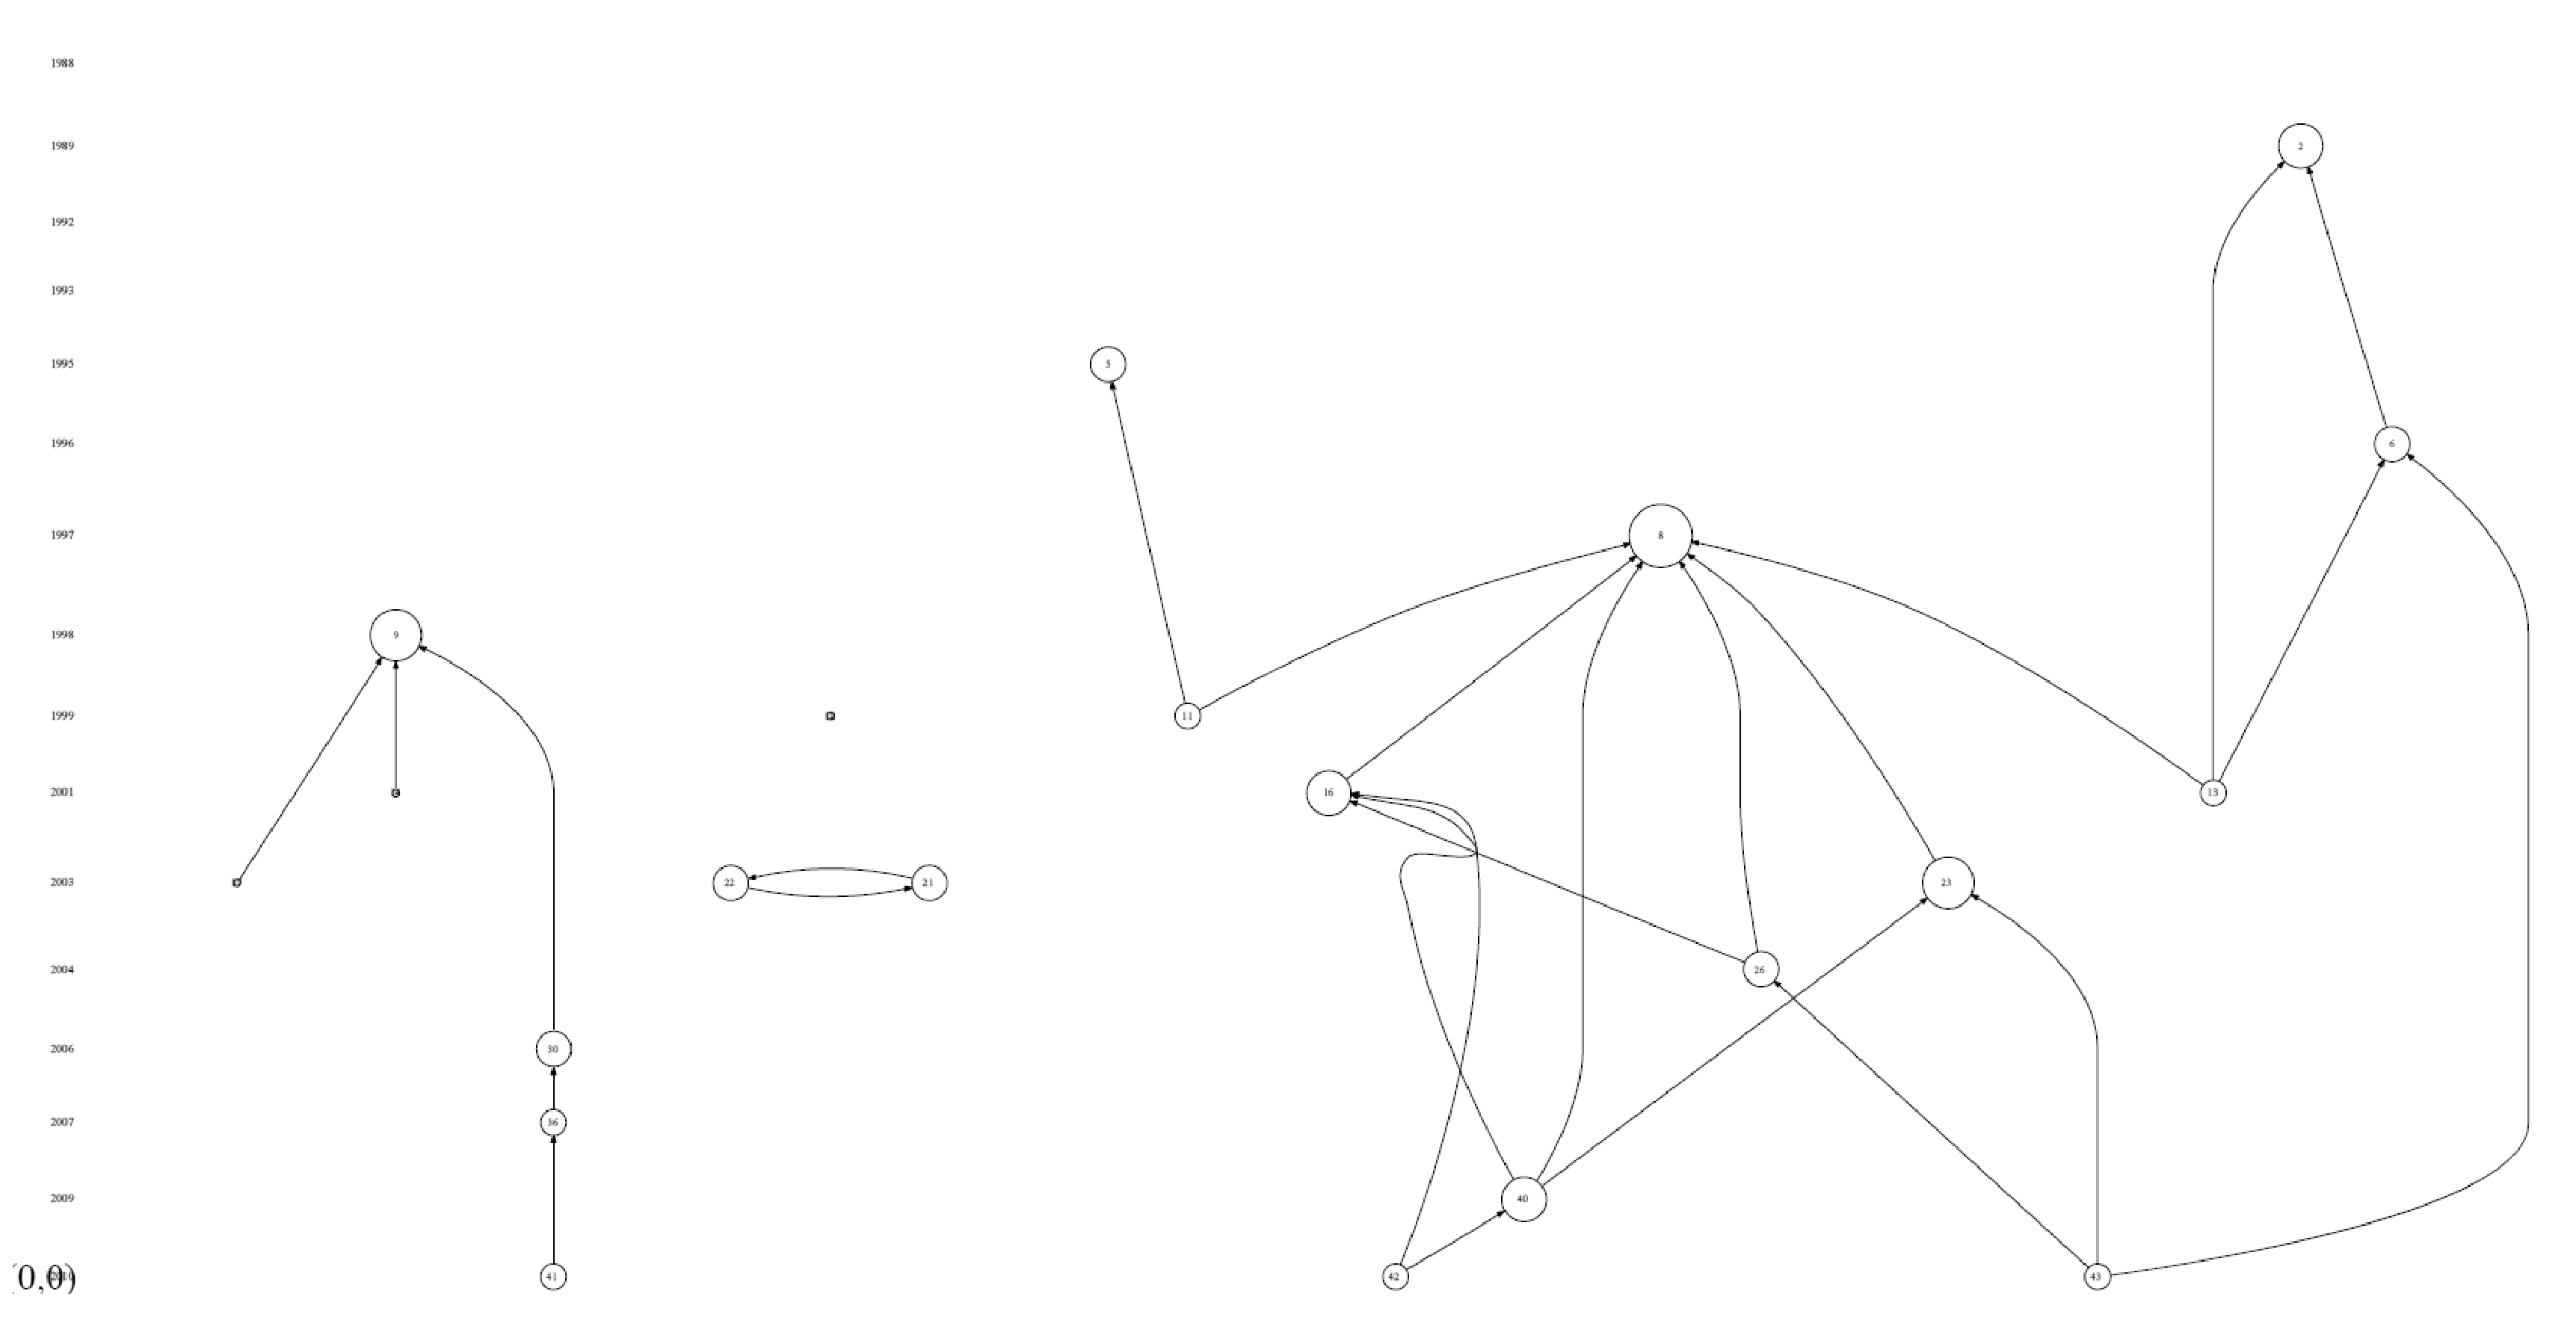
\includegraphics[width=18cm,height=13cm]{LCS.eps}
		\end{center}
	\section{GCS图}
	\begin{center}
		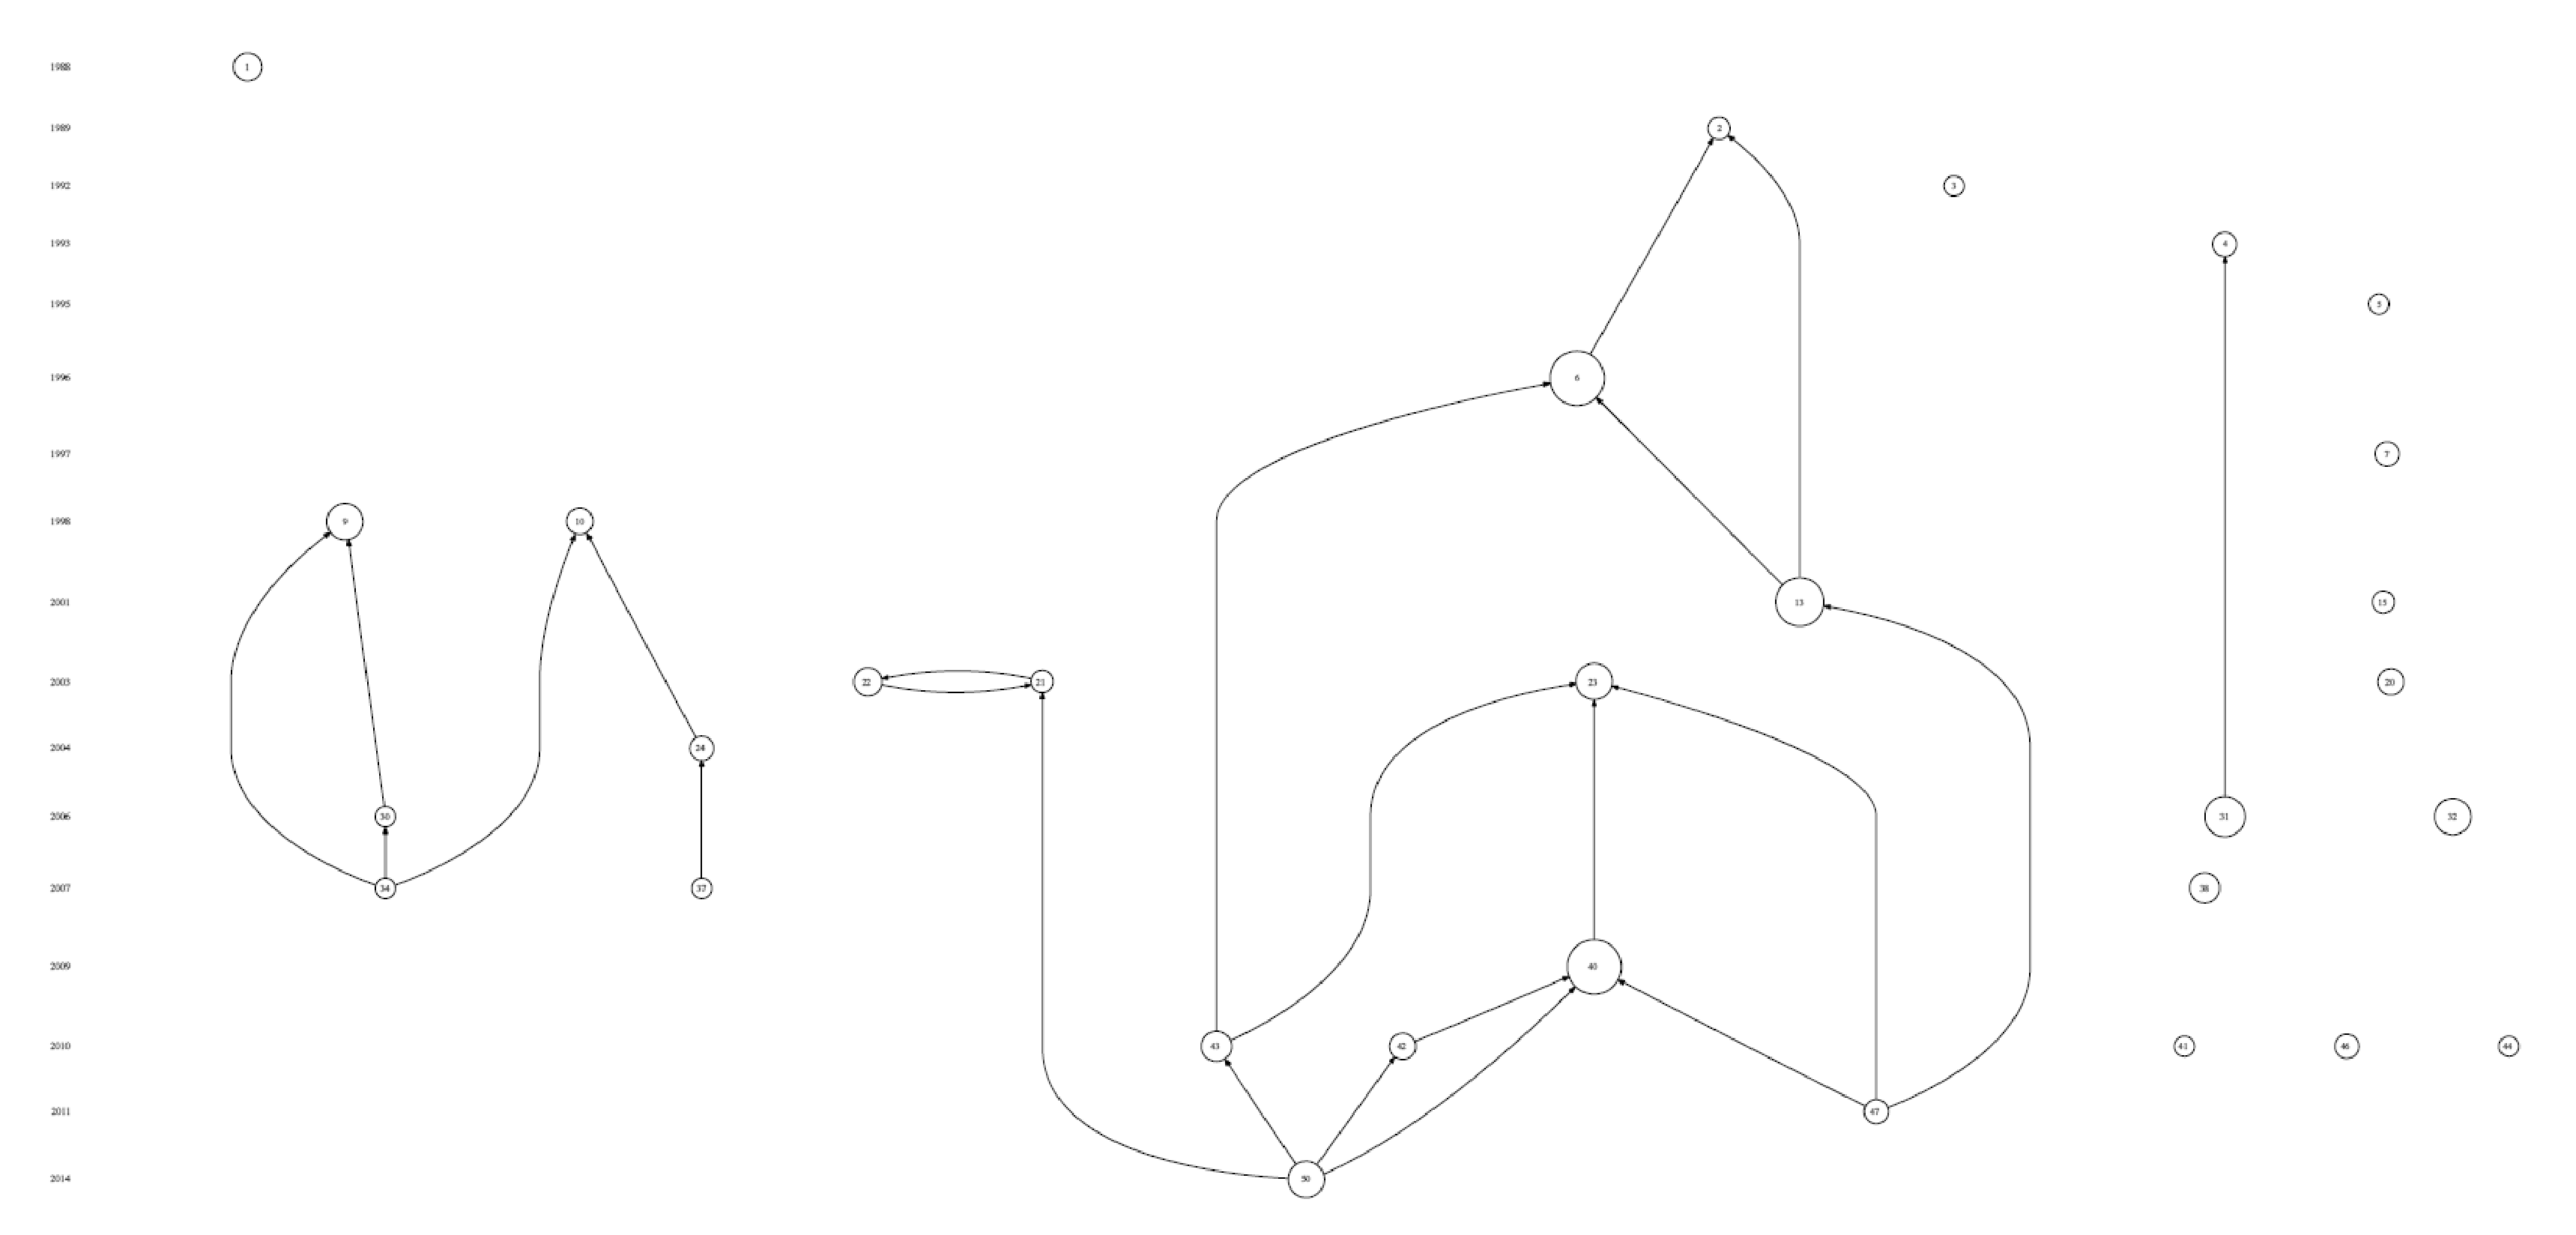
\includegraphics[width=18cm,height=13cm]{GCS.eps}
	\end{center}
\section{分析}
从上面的LCS图中可以看到,先看左边的年份从1988~2009,现在是2018年,最近几年没有高被引文章,说明这个领域已经不是那么活跃了。再看这个图,可以看到文章8被引的最多,这个文章可能做了一些开创性的工作,文章的引用大致分了三部分,主要的是最右边的部分互相引用情况较明显,在中间的21和22就只是互相引用。从GCS中可以看到,文章6和文章40的圈最大,也就是被引次数多,文章6跟LCS的情况并不是非常一致,说明可能这篇文章引起了别的领域的关注而在本领域内得到了并不是那么多的关注。
\section{比较}
用HistCite作文献分析的过程其实应该是很不错的,因为它更加直观的提供了一些分析,把文章之间的关联都画在了图上,正所谓一图胜千言\smiley,这大大缩短了我们找到核心文献或者重要文献的时间。但是我觉得用户体验并不好,首先要导出文章,然后拖入分析,分析的过程又可能出意外,比如我就拖不进去要放到txt文件夹\frownie,在画图中点击导出经常ie就卡,导\cite{lamport94}出的格式为什么也是ps的,我插不进去文档啊。

但是,总的来说优点大于缺点,因为前面被省略的时间还是大于后面花费的时间。所以,这也是一个不那么锋利的科研工具。
\begin{thebibliography}{9}
	
	\bibitem{lamport94}
	Leslie Lamport,
	\textit{\LaTeX: a document preparation system},
	Addison Wesley, Massachusetts,
	2nd edition,
	1994.
	
\end{thebibliography}
\end{document}